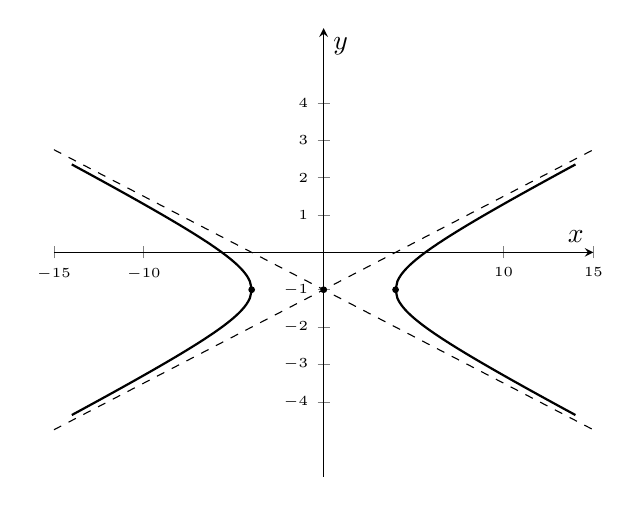
\begin{tikzpicture}

    % Configura os eixos com limites de -15 a 15
    \begin{axis}[
            axis lines=middle, % Eixos no meio
            xlabel={$x$}, % Rótulo do eixo x
            ylabel={$y$}, % Rótulo do eixo y
            xmin=-15, xmax=15, % Limites do eixo x
            ymin=-6, ymax=6, % Limites do eixo y
            xtick={-15,-10,10,15}, % Marcadores do eixo x
            ytick={-4,-3,...,3,4}, % Marcadores do eixo y
            tick label style={font=\tiny}, % Tamanho da fonte dos ticks (muito 
            % domain=4:9, % Domínio da hipérbole
            samples=100, % Número de amostras para a curva
            legend style={at={(1.05,1)}, anchor=south west}, % Estilo da legenda
        ]

        % Desenha a hipérbole, separando os ramos
        \addplot[thick, domain=4:14] {-1 + sqrt((x)^2/16 - 1)}; % Ramos superiores
        \addplot[thick, domain=4:14] {-1 - sqrt((x)^2/16 - 1)}; % Ramos inferiores

        % Desenha a hipérbole, separando os ramos
        \addplot[thick, domain=-14:-4] {-1 + sqrt((x)^2/16 - 1)}; % Ramos superiores
        \addplot[thick, domain=-14:-4] {-1 - sqrt((x)^2/16 - 1)}; % Ramos inferiores

        % Desenha as assíntotas
        \addplot[dashed, domain=-15:15] {-1 + 0.25*x}; % Assíntota superior
        \addplot[dashed, domain=-15:15] {-1 - 0.25*x}; % Assíntota inferior

        % Marca os vértices
        \filldraw[black] (4,-1) circle (1pt);
        \filldraw[black] (-4,-1) circle (1pt);
        \filldraw[black] (0,-1) circle (1pt);




    \end{axis}

\end{tikzpicture}